\documentclass[tikz,border=2pt]{standalone}
\usepackage{tikz}
\begin{document}
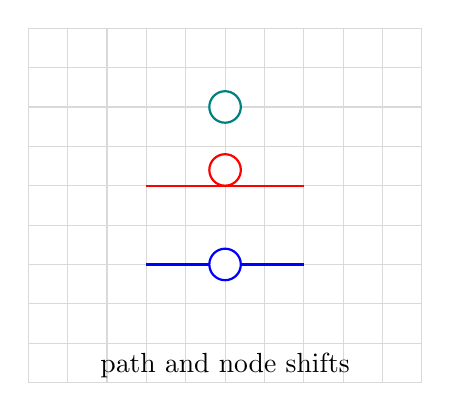
\begin{tikzpicture}
  \draw[gray!30,step=.5cm] (-.5,-.5) grid (4.5,4);
  \draw[xshift=1cm,yshift=1cm,blue,thick]
    (0,0) -- node[draw,circle,fill=white,inner sep=0pt,minimum size=4mm] (a) {} (2,0);
  \draw[shift={(1,2)},red,thick]
    (0,0) -- node[draw,circle,fill=white,inner sep=0pt,minimum size=4mm,yshift=2mm] (b) {} (2,0);
  \coordinate (p) at (2,3);
  \draw[xshift=1cm,teal,thick] (1,3) -- (p)
    node[draw,circle,fill=white,inner sep=0pt,minimum size=4mm] (c) {};
  \node[below] at (2,0) {path and node shifts};
\end{tikzpicture}
\end{document}
